\chapter{Structure learning}\label{chp:structure}

In this chapter we cover two structure learning algorithms we use for image classification. The
first is based on~\cite{clustering}. The second is a variation of~\cite{gens-domingos}'s structure
learning schema. Once we cover both algorithms, we explain how we add a slight modification to the
first architecture. We have empirically found that this change increased image classification
accuracy significantly. We call this the ``classification architecture''.

\section{The Dennis-Ventura architecture}

Let us first formalize the notion of dataset. We call a dataset a set of \textit{instances}, where
each instance is a set we call \textit{valuation} or \textit{instantiation}. As we have mentioned
before, a valuation may be incomplete, meaning that an instantiation of some random variable may be
missing from the instance. In this thesis we assume complete data, as both structure learning
algorithms do not admit incomplete datasets.

Having said that, let $D$ be a complete dataset. Since $D$ is complete, for each instance $I$ we
can map each random variable $X$ from $I$ to a number, yielding an ordered vector $(X_1,X_2,\ldots,
X_m)$ equivalent to $I$. We do the same for each instance $I$. The vector $(I_1,I_2,\ldots, I_n)$
is a representation of $D$. This way, $D$ could be seen as a $m\times n$ matrix. We denote by
$D^\intercal$ the transpose of the matrix representation of the dataset $D$.  Let $T$ be a
subscope, that is, a subset of the set of all variables in the SPN\@. We use the notation $D_T$ to
represent the matrix of all instances from $D$ but restricted only to elements from random
variables in $T$.

Since we are restricted to the image classification domain, we give some semantic meaning to
datasets. If $D$ is a dataset, then each instance $I\in D$ can be seen as a vector containing all
the pixel values of an image plus a classification label. Each variable is a pixel from the image,
and each variable value is the pixel's color intensity. If the dataset $D$ is a vector of images
and their labels, the transpose $D^\intercal$ is a vector of variables and their values in each
image.

Just like in~\cite{poon-domingos}, the Dennis-Ventura algorithm uses the notion of similarity
between local variables.  This local neighborhood is called a Region. A Region represents a cluster
of pixels that has some semantic value when grouped together. Contrastingly, a Decomposition
represents independence between variables. In an SPN, a Region is graphically represented by a set
of sum nodes, whilst a Decomposition is a set of products.

To learn an SPN structure from data,~\cite{clustering} uses a \textit{region graph}, which is a
simplified representation of an SPN made out of Region nodes and Decomposition nodes.

\begin{figure}[h]
  \begin{subfigure}{.4\linewidth}
    \centering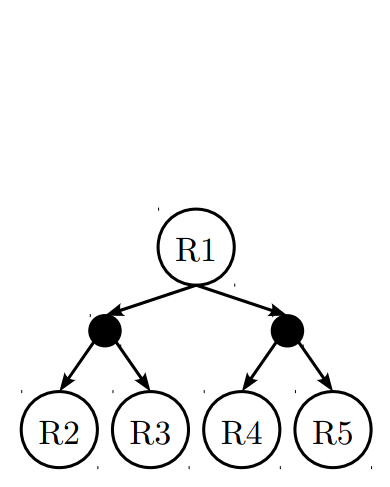
\includegraphics[scale=1.0]{imgs/simple_dv.png}
    \caption{}
  \end{subfigure}
  \begin{subfigure}{.6\linewidth}
    \centering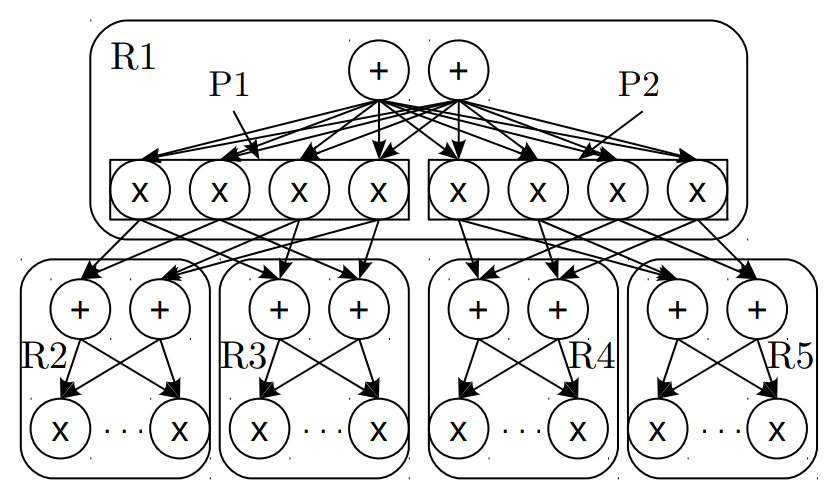
\includegraphics[scale=1.0]{imgs/trans_dv.png}
    \caption{}
  \end{subfigure}
  \caption{Dennis-Ventura region graph and translated SPN as shown in~\cite{clustering}.}
\end{figure}

The region graph is generated by recursively finding two subregions from a parent region through
the use of $k$-means clustering. Let $R$ be a region, and $D_R^\intercal$ the transposed dataset
restricted to $R$'s scope. We partition $R$ into two subregions $R_1$ and $R_2$ by $k$-means
clustering $D_R^\intercal$, yielding two subclusters $D_{R_1}^\intercal$ and $D_{R_2}^\intercal$.
We then apply recursion on the two subregions. At each clustering step, we connect regions $R$ to a
decomposition node $P$, which is then connected to each $R_i$ node. Our stop criteria is when
$\Sc(R_i)=1$.

Once created, the region graph is then translated to a valid SPN\@. Each region node $R$ is
translated to a set of SPN nodes. If $\Sc(R)=1$, then these nodes are $g$ univariate gaussian
distributions, where each gaussian is a different quantile of the distribution of the pixel. Else,
$m$ sum nodes are created. Partition nodes are translated to product nodes. Edges are added such
that every product child node of a region is connected to all sum nodes in the region. Each of
these product nodes are then connected to a distinct pair of sum nodes from both region's children
subregions, meaning that each decomposition node contains $2^m$ products.

With the architecture done, we apply parameter learning on the SPN to learn weights. This is done
either through gradient descent or EM\@. In this thesis we apply generative and discriminative
gradient descent to the architecture.

\section{The Gens-Domingos schema}

In~\cite{gens-domingos}, Gens and Domingos describe a flexible schema for structure learning of
SPNs. The schema is based on the idea that the scope in a sum node's child mean that these
variables are similar (and by consequence dissimilar to the variables in other sibling nodes'
scopes), and that variables in a product's child mean that variables are dependent of each other
(and analogally to sums, independent of other siblings).

This interpretation of SPNs yields an adaptable and open schema of learning. Sum nodes are created
through clustering, as each cluster has some similarity aspect given some metric. Meanwhile,
product nodes are created through statistical variable independence algorithms. When the scope of
this partitioning of variables is one, we create a univariate distribution over the partitioned
dataset.

\begin{algorithm}[H]
  \caption*{\code{GensArch}: Gens-Domingos structure learning schema}
  \begin{algorithmic}[1]
    \Require Set of instances $D$ and scope $X$
    \Ensure SPN structure learned from $D$ and $X$
    \If{$|X|=1$}
      \State \textbf{return} univariate distribution over $D_X$
    \Else%
      \State Partition $X$ into $P_1,P_2,\ldots,P_m$ such that every $P_i$ is independent of $P_j$,
        $i\neq j$
      \If{$m>1$}
        \State Let $\pi$ be a new product node
        \For{$i\gets 1,\ldots,m$}
          \State $p_i\gets$\code{GensArch}$(D_{P_i}, P_i)$
          \State $\pi$\code{.AddChild}$(p_i)$
        \EndFor%
        \State \textbf{return} $\pi$
      \Else%
        \State Cluster $D$ such that $Q_1,Q_2,\ldots,Q_n$ are $D$'s clusters
        \State Let $\sigma$ be a new sum node
        \For{$i\gets 1,\ldots,n$}
          \State $s_i\gets$\code{GensArch}$(Q_i, X)$
          \State $w\gets |Q_i|/|D|$
          \State $\sigma$\code{.AddChild}$(s_i, w)$ \Comment{$w$ is edge $\sigma\to s_i$'s weight}
        \EndFor%
        \State \textbf{return} $\sigma$
      \EndIf%
    \EndIf%
  \end{algorithmic}
\end{algorithm}

Our implementation was done by using DBSCAN, a density based clustering algorithm that
automatically decides the number of clusters to generate (\cite{dbscan}), for clustering and the
traditional G-test for variable independence. We additionally implemented $k$-means, $k$-mode and
$k$-median for clustering and Pearson's $\chi^2$-square for independence testing. However, we found
that DBSCAN yielded the best clustering results and G-test the best variable independence.

For variable independence, instead of testing every variable pairwise, we constructed a dependency
graph. Each vertex from the dependency graph represents a variable. An edge between two vertices
means the two variables are dependent. To find independent partitions in a dataset it suffices to
find a spanning tree of the dependency graph. We do this through Kruskal's MST union-find
algorithm. The resulting connected components of the spanning tree are the partitions we wish to
find. This significantly reduces complexity. However, we have found that it still accounts for
approximately 90\% of the algorithm's runtime.

We conjecture that a better approach to variable indepedence would be finding approximate spanning
trees on the graph. Many independence tests resulted in a completely dependent graph, but with
cuts that could possibly yield better accuracy and runtime performance.

\section{The classification architecture}


